\section{Gestion des paires}

\textbf{Si vous êtes membres du staff, et que vous avez la permission de gérer les paires}, vous pouvez alors accéder à la page de gestion des paires, depuis l'onglet "Staff" tout à droite du menu de navigation.

\begin{figure}[H]
\centering
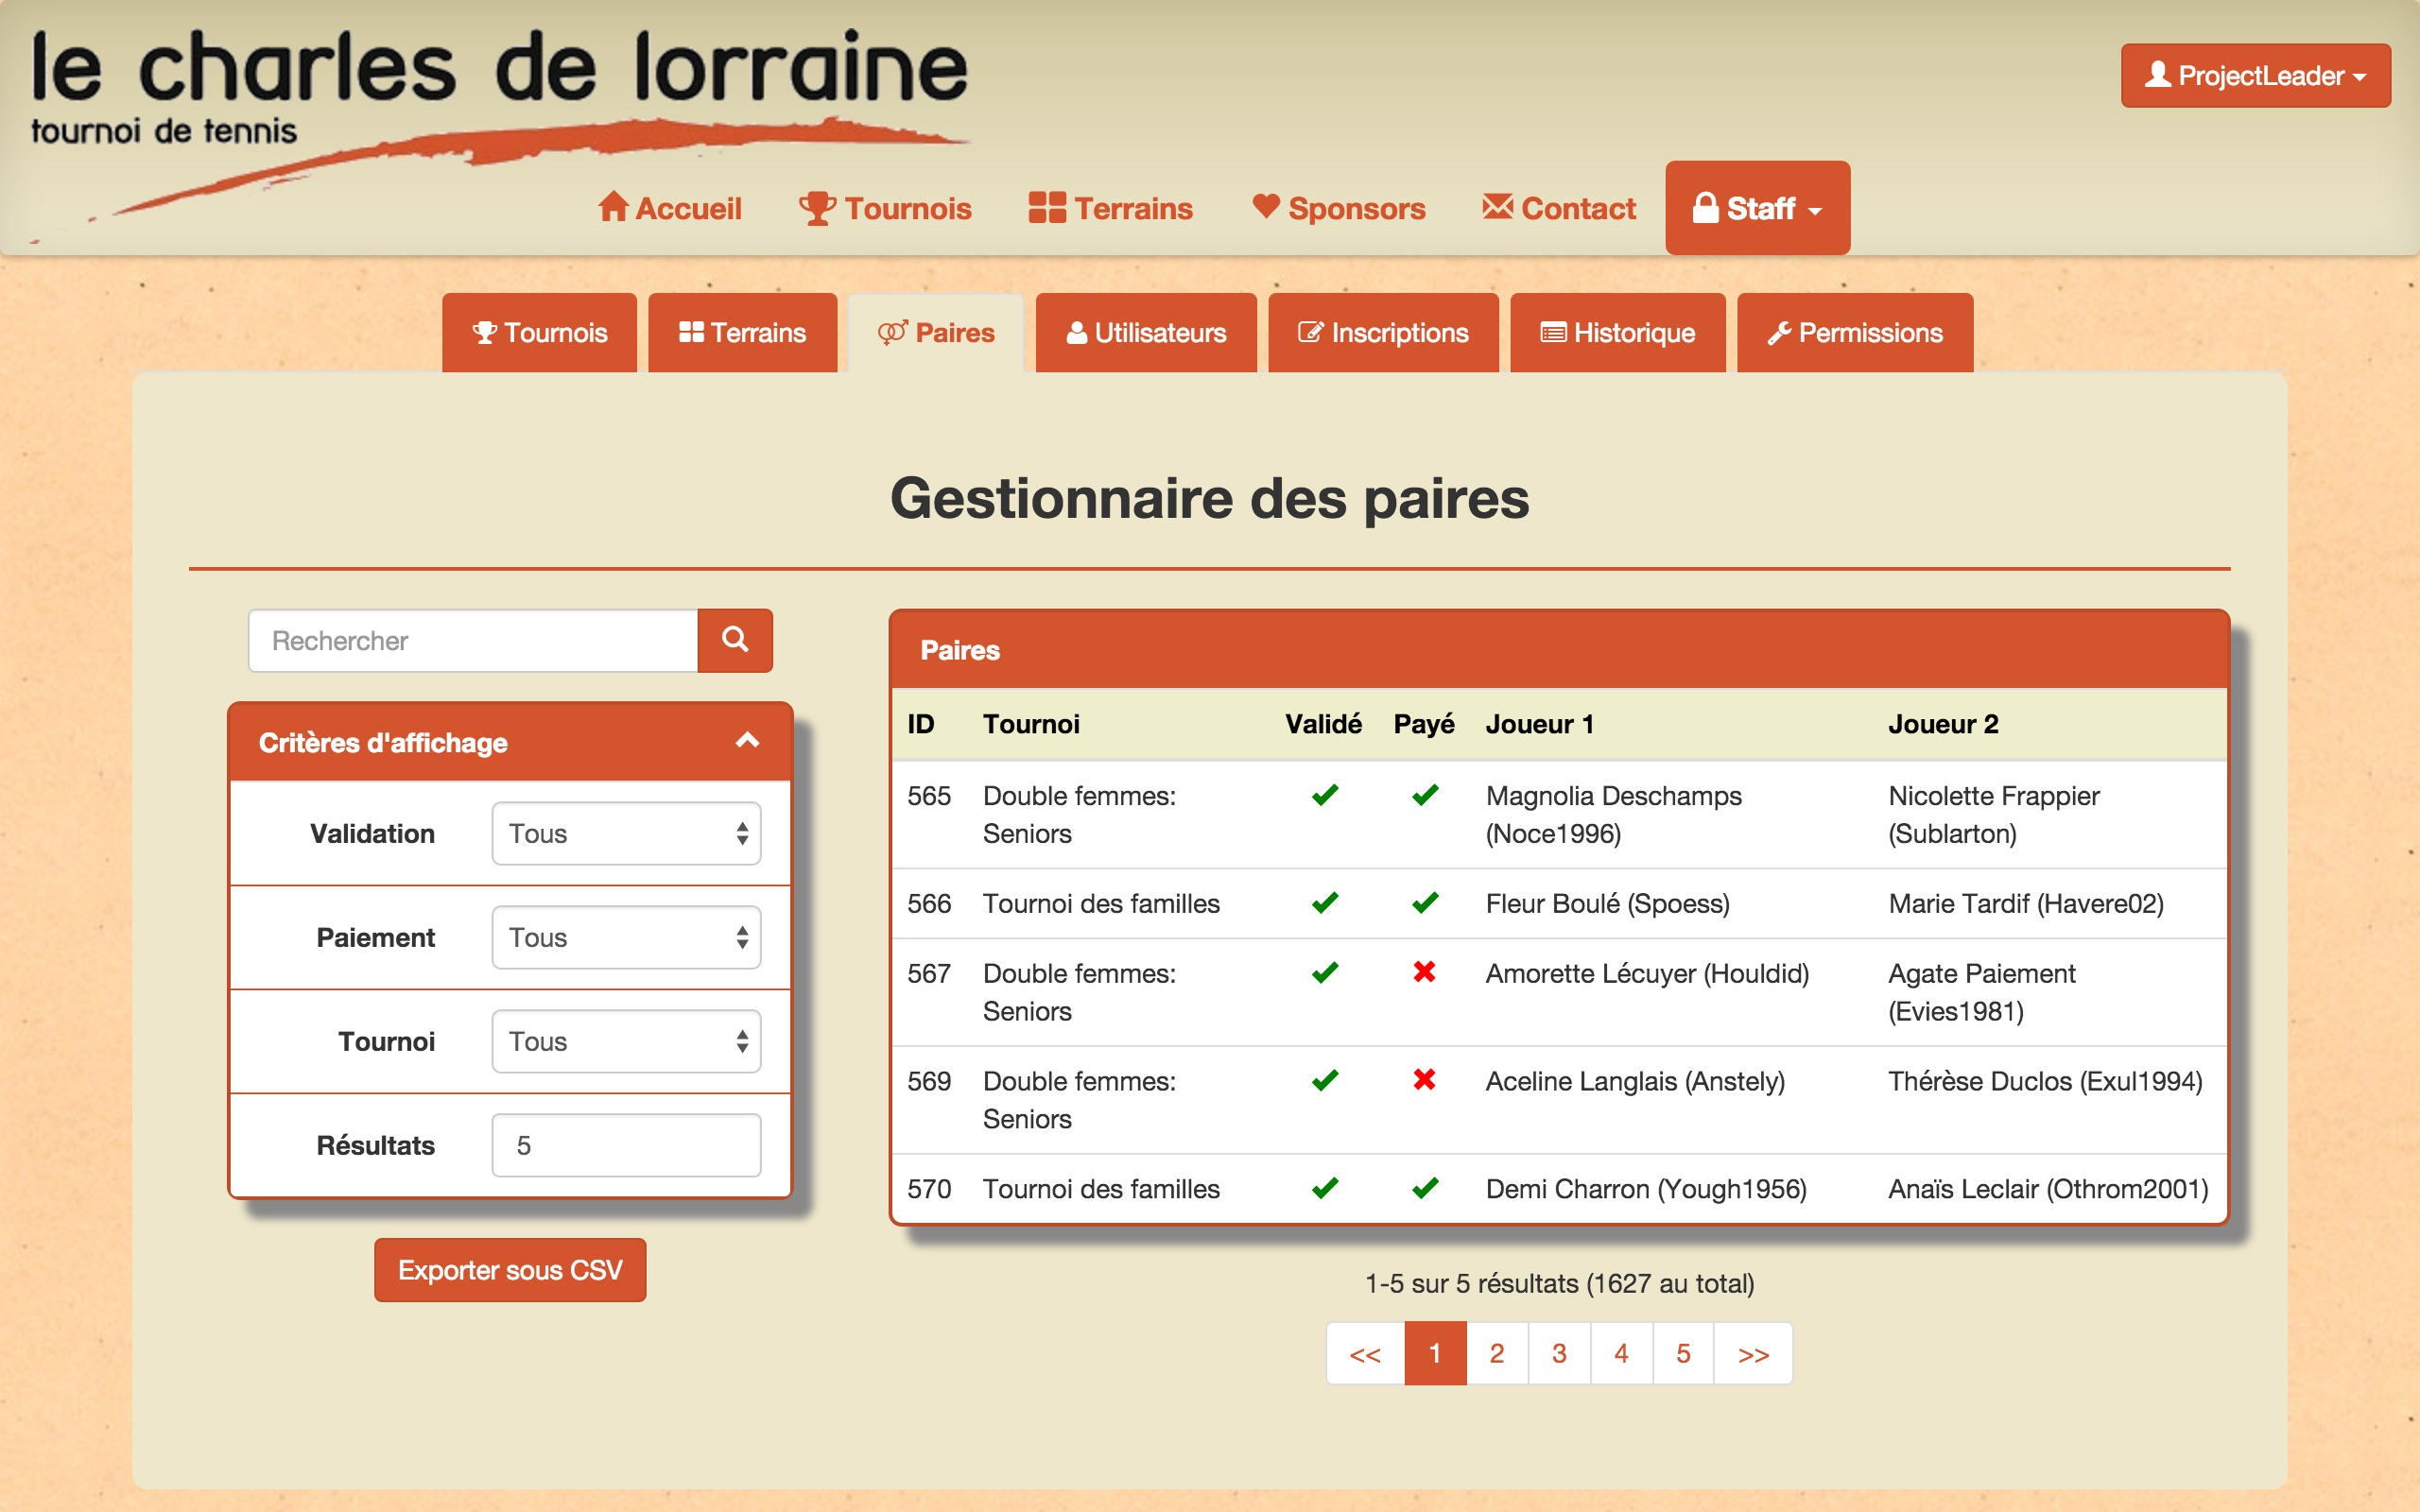
\includegraphics[scale=0.15]{gestion-paires/gestion-paires.jpg}
\caption{Page staff principale pour la gestion des paires}
\end{figure}

\subsection{Les paires}

Depuis la page staff "Gestionnaire des paires", vous pouvez gérer toutes les paires qui se trouve dans la base de données. Pour donner la permission à un utilisateur de gérer les paires, l'admin doit lui octroyer les permissions à partir de la page "Gestionnaire des permissions"

% TODO
\todo[inline]{Ajouter une référence vers la page Gestionnaire des permissions}
\bigskip

Sur cette page, vous pouvez rechercher des paires, consulter une paire, la valider, la signaler comme ayant payée l'inscription, et la supprimer.\newline

La page principale de la gestion des paires est divisée en 2 parties :

\begin{itemize}
\item  à gauche, un champ et des critères de recherche, et un bouton pour exporter la liste des terrains au format CSV ;
\item à droite, la liste des paires qui respectent les critères choisies, et possédant certaines données qui ont une correspondance partielle avec le texte entré dans le champ de recherche ;
\end{itemize}
\bigskip

Les critères d'affichage des paires sont les suivants :

\begin{itemize}
\item \textbf{Validation} : permet de filter les paires selon qu'elles aient été validées par le staff ou non (oui, non, tous)
\item Paiement : permet de filter les paires selon qu'elles aient été indiquées comme ayant payé les frais d'inscription et les extras choisies ou non (oui, non, tous)
\item Tournoi : permet de filter les paires selon le tournoi d'inscription (Double mixte : pre-minimes, Tournoi des familles, ...)
\item \textbf{Résultats} : permet d'indiquer le nombre de paires à afficher à la fois par page dans la liste des paires à droite
\end{itemize}
\bigskip

Pour effectuer une recherche, il faut sélectionner les critères et entrer le champ de recherche souhaité, puis valider la recherche en cliquant soit sur le bouton de la loupe, soit en appuyant sur la touche \textit{Entrée} du clavier. Le module des critères de recherche peut être minimisé, à tout moment, en cliquant sur le bouton dans le coin droit supérieur du module en forme de "V" (inversé si la liste des critères sont visibles).\newline

Pour consulter une paire, il suffit de cliquer sur l'entrée de la liste des paires contenant les informations de la paire que l'on souhaite consulter. Par exemple, pour consulter la paire avec l'ID 565, il suffit de cliquer sur la ligne de la liste des paires où la valeur 565 se trouve dans la colonne ID.

\subsection{Gestion d'une paire}

\begin{figure}[H]
\centering
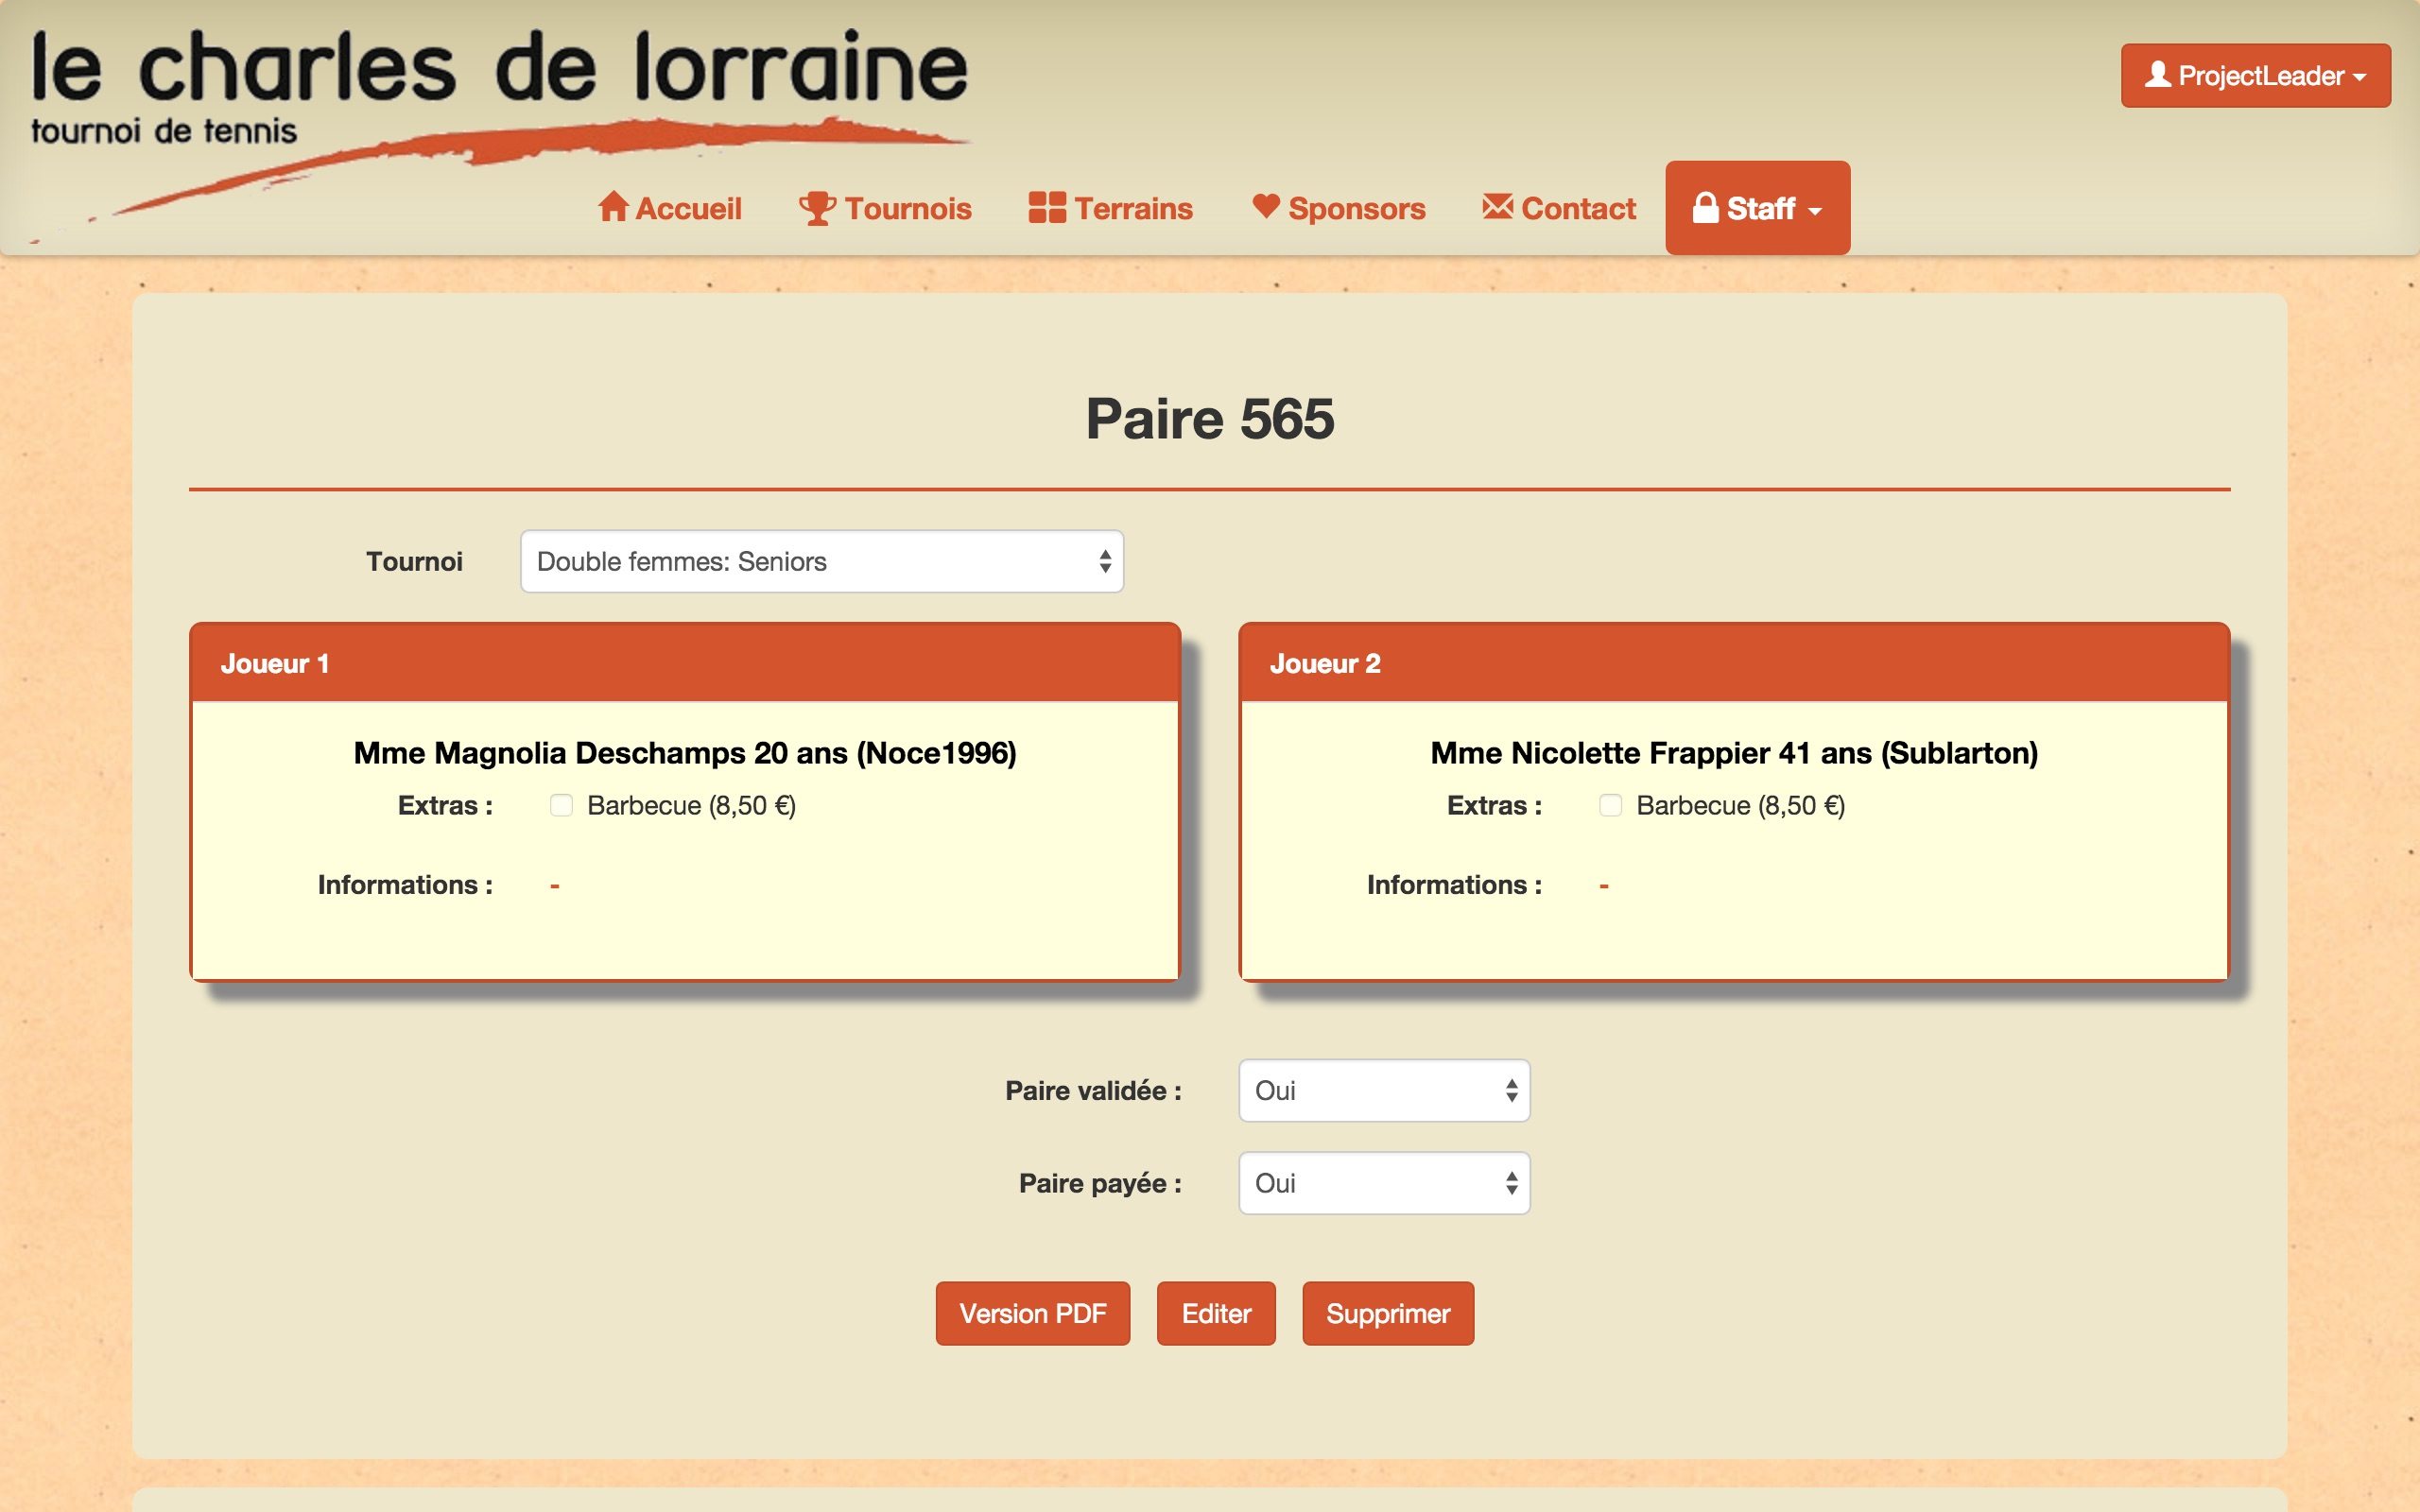
\includegraphics[scale=0.15]{gestion-paires/gestion-paires-paire.jpg}
\caption{Page staff de la gestion d'une paire}
\end{figure}

La page de gestion d'une paire se présente en deux modules, un par joueur, contenant les extras choisis et les commentaires des joueurs. La liste déroulante en haut de la page permet de sélectionner le tournoi de la paire, permettant facilement d'inscrire la paire à un autre tournoi que celui initialement indiqué.\newline

Pour indiquer que les paires sont éligibles au tournoi, il faut les valider en sélectionnant "Oui" dans la liste déroulante de "Paire validée", en dessous des modules des informations des joueurs. Pour indiquer que la paire a bien payé son inscription, il faut sélecitonner "Oui" dans la liste déroulante de "Paire payée". Pour confirmer ces changements, il faut cliquer sur le bouton \textit{Editer} en bas de la page.\newline

En plus du bouton \textit{Editer}, qui permet d'appliquer les modifications apportées à la paire, deux autres boutons permettent de télécharger les informations de la paire au format PDF (\textit{Version PDF}), et de supprimer définitivement la paire (\textit{Supprimer}). Puisque cette dernière action est irréversible, une boîte de dialogue demande à l'utilisateur de confirmer son choix de supprimer la paire.
